\section{Hàm lồi mở rộng}
\begin{dn}
Cho hàm $f: S \rightarrow [-\infty, \infty]$ trên tập $S \subset \R ^n$ khác rỗng, hàm $f$ được gọi là lồi trên $S$ nếu và chỉ nếu với bất kỳ $x^1, x^2 \in S$ và $\lambda \in [0,1]$, ta có:
\begin{equation*}
    f(\lambda x^1 +(1-\lambda) x^2) \leq \lambda f(x^1) + (1 - \lambda) f(x^2)
\end{equation*}
Mặt khác, một hàm $f$ được gọi là lõm trên $S$ nếu $-f$ là lồi trên $S$.
\end{dn}
\begin{dn}
    Cho hàm $f: S \rightarrow [-\infty, \infty]$ trên tập $S \subset \R ^n$ khác rỗng, hàm $f$ được gọi là tựa lồi (quasiconvex) trên $S$ nếu và chỉ nếu với bất kỳ $x^1, x^2 \in S$ và $\lambda \in [0,1]$, ta có:
    \begin{equation*}
         f(\lambda x^1 + (1 - \lambda)x^2) < \max \{f(x^1), f(x^2)\}
     \end{equation*}
     hay một cách tương đương:
     \begin{equation*}
          f(x^1) \geq f(x^2) \Rightarrow f(x^1) \geq f(x^1 + \lambda(x^2 - x^1))
     \end{equation*}
\end{dn}

\begin{dn}
    Với mỗi số thực $\alpha \in \R$, ta gọi
    $$ L_\alpha(h) := \{x \in S\ |\ f(x) \leq \alpha \} $$
    là tập mức dưới của hàm $f$ và
    $$ L^\alpha(h) := \{x \in S\ |\ f(x) \geq \alpha \} $$
    là tập mức trên của hàm $f$.
\end{dn}

\begin{dl}[\cite{gen_convex}]
    \label{quasiconvex_theo}
    Hàm $f$ xác định trên tập lồi $S \subseteq \R^n$ khác rỗng là hàm tựa lồi khi và chỉ khi tập mức dưới $L_\alpha$ của hàm đó lồi với mọi $\alpha \in \R$
\end{dl}
\begin{vd}
    Xét hàm số
    \begin{equation*}
        h(x) = \sqrt{|x|}
    \end{equation*}
    trên tập $\R$
\end{vd}
\begin{figure}
    \centering
    \begin{tikzpicture}[declare function={f(\x)=sqrt{abs(\x};}]
    \begin{axis}[
            width=0.8\textwidth,
            height=0.6\textwidth,
            axis on top,
            legend pos=outer north east,
            axis lines = center,
            % xticklabel style = {font=\tiny},
            % yticklabel style = {font=\tiny},
            xlabel = $x$,
            ylabel = $y$,
            legend style={cells={align=left}},
            legend cell align={left},
        ]
        \addplot[very thick,red,samples=161,domain=-3:3,name path=f] {f(x)};
        \addplot[very thick,red,samples=161, domain=-2:2, name path=g]
        {sqrt(2)};
        \addplot[red!10, opacity=0.4] fill between[of=f and g, soft clip={domain=-2:2}];
    \end{axis}
\end{tikzpicture}
    \caption{: Đồ thị của hàm số $h(x) = \sqrt{|x|}$ trên tập số thực $\R$}
    \label{fig:vd1.1}
\end{figure}
Dễ thấy mọi tập mức dưới $L_\alpha(h)$ của $h(x)$ đều là tập lồi (xem Hình
\ref{fig:vd1.1}) nên $h(x)$ là hàm tựa lồi trên $\R$.

\begin{vd} \label{vd:1.2}
    Xét hàm số $$h(x;y) = -xy$$ xác định trên $S = \{(x,y) \in \R^2 | x, y \geq 0 \}$
\end{vd}

\begin{figure}
    \centering
    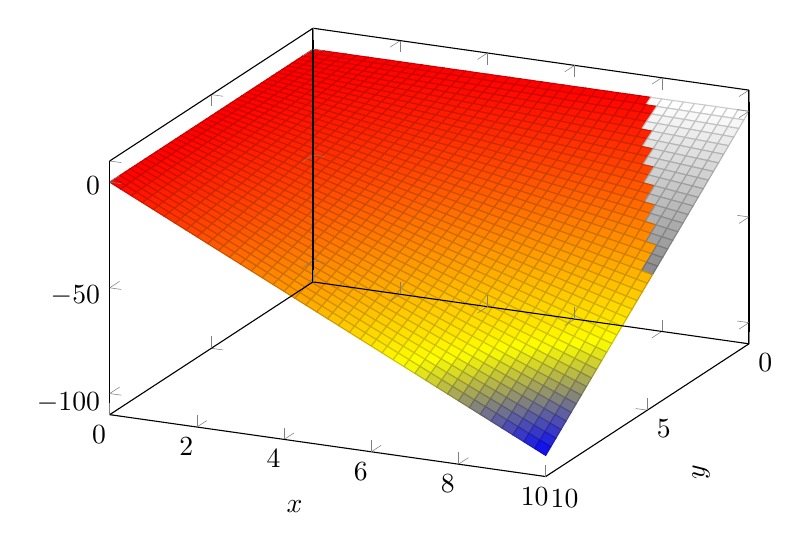
\begin{tikzpicture}
        \begin{axis}[
            %hide axis,
            width=0.8\textwidth,
            height=0.6\textwidth,
            axis on top,
            axis lines = box,
            xlabel=$x$,ylabel=$y$,
            y dir = reverse,
                    mesh/interior colormap name=hot, colormap/blackwhite,
                    ]
            \addplot3[domain=0:10,surf,samples=41] {-x*y};
        \end{axis}
    \end{tikzpicture}
    \caption{: Đồ thị của hàm số $ h(x, y) = -xy$ trên $[0, 10]^2$}
    \label{fig:vd1.2}
\end{figure}

Với $\alpha$ bất kỳ thuộc $\R$ ta có tập mức dưới của $h$
\begin{equation*}
    L_\alpha(h) = \{(x, y) \in S | -xy \leq \alpha \} = \{(x, y) \in \R^2| x, y \geq 0, xy \geq -\alpha\}
\end{equation*}

\begin{vd}
    Xét hàm số
    \begin{equation*}
        h(x, y) = xy + x^2y^2 + x^3y^3
    \end{equation*}
    xác định trên $\R^2_+$
\end{vd}
\begin{figure}[h!]
    \centering
    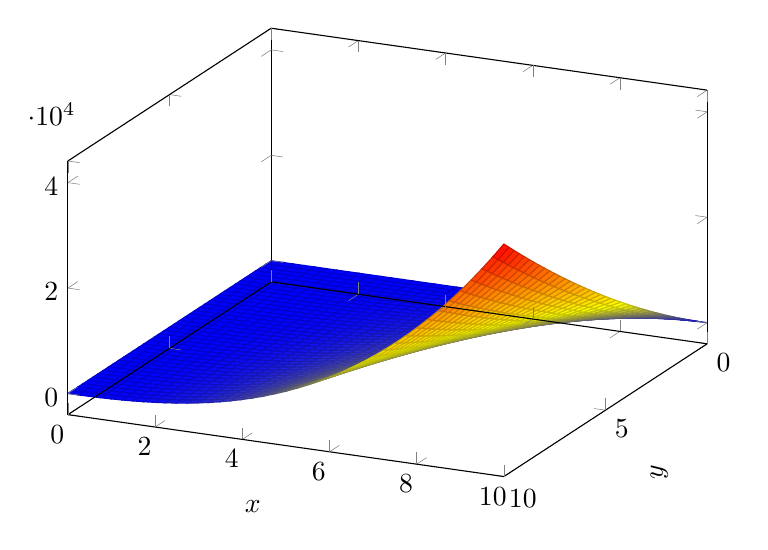
\begin{tikzpicture}
        \begin{axis}[
            %hide axis,
            width=0.8\textwidth,
            height=0.6\textwidth,
            axis on top,
            axis lines = box,
            xlabel=$x$,ylabel=$y$,
            y dir = reverse,
                    mesh/interior colormap name=hot, colormap/blackwhite,
                    ]
            \addplot3[domain=0:10,surf,samples=41] {x*y + x^2*y^2 + x^3*y*3};
        \end{axis}
    \end{tikzpicture}
    \caption{: Đồ thị của hàm số $ h(x, y) = xy + x^2y^2 + x^3y^3$ trên $[0, 10]^2$}
    \label{fig:vd1.3}
\end{figure}
Đặt $g(t) = t + t^2 + t^3$ và $u(x, y) = xy$ thì $ h(x, y) = g(u(x, y))$. Từ Ví dụ \ref{vd:1.2}, ta có $-xy$ là hàm tựa lồi nên $u(x, y) = xy$ là hàm tựa
lõm. Do $g$ là hàm không giảm và $u$ là hàm tựa lõm trên $S$ nên $h$ là một
hàm tựa lõm trên $S$ (xem [2], tr. 57).

\begin{dn}
     Cho hàm $f: S \rightarrow [-\infty, \infty]$ trên tập $S \subset \R ^n$ khác rỗng, hàm $f$ được gọi là tựa lồi chặt (strictly quasiconvex) nếu và chỉ nếu với bất kỳ $x^1, x^2 \in S$, $x^1 \neq x^2$ và $\lambda \in [0,1]$, ta có:
     \begin{equation*}
         f(\lambda x^1 + (1 - \lambda)x^2) < \max \{f(x^1), f(x^2)\}
     \end{equation*}
     hay một cách tương đương:
     \begin{equation*}
          f(x^1) \geq f(x^2) \Rightarrow f(x^1) \geq f(x^1 + \lambda(x^2 - x^1))
     \end{equation*}
\end{dn}

\begin{vd}
Hàm 
$
f(x) = 
\begin{cases}
\dfrac{|x|}{x}, &x \neq 0 \\
0, & x = 0
\end{cases}
$
là hàm tựa lồi nhưng không tựa lồi chặt.
\end{vd}
Ta biết rằng điểm cực trị của một hàm lồi đồng thời là cực tiểu toán cục của hàm đó. Tuy nhiên, tính chất này không chỉ đúng với các hàm tựa lồi và tựa lồi chặt, vì vậy một lớp hàm mới được giới thiệu:
\begin{dn}[xem \cite{gen_convex}]
    \label{psuedoconvex_def}
    Cho một hàm $f$ khả vi trên một tập lồi mở $S \subset \R^n$, hàm $f$ được gọi là giả lồi trên $S$ khi và chỉ khi:
    \begin{equation}
    \label{dn1}
    x^1, x^2 \in S, f(x^1) > f(x^2) \Rightarrow \nabla f(x^1)^T (x^2 - x^1) < 0
    \end{equation}
\end{dn}
Nếu bất đẳng thức trong vế phải của \eqref{dn1} vẫn đúng trong trường hợp $f(x^1) = f(x^2)$ thì $f$ được gọi là giả lồi chặt (strictly psuedoconvex), hay phát biểu một cách đầy đủ như sau:
\begin{dn}
    Một hàm $f$ khả vi trên một tập lồi mở $S \subset \R^n$ được gọi là giả lồi chặt (strictly psuediconvex) trên $S$ khi và chỉ khi:
    \begin{equation*}
        x^1, x^2 \in S,\ x^1 \neq x^2,\ f(x^1) > f(x^2) \Rightarrow \nabla f(x^1)^T (x^2 - x^1) < 0
    \end{equation*}
\end{dn}

\begin{md}[\cite{Clarke1983}]
    \label{normal_cone_prop}
    Giả sử tập khác rỗng $\Omega \subset \R^n$ lồi và đóng. Ta định nghĩa nón pháp tuyến của $\Omega$ tại $x \in \Omega$ là tập các vector thỏa mãn,
    \begin{equation*}
        N_\Omega(x) = \left\{ v \in \R^n: v^T(x - x^\prime) \geq 0,\ \forall x^\prime \in \Omega \right\}
    \end{equation*}
    Nếu $G: \R^n \to \R$ liên tục Lipschitz tại lân cận $x$ và đại cực tiểu tại $x$, thì $0 \in N_\Omega(x) + \partial G(x)$
\end{md}

\begin{md}[\cite{gen_convex}]
    \label{md_quasi}
    Nếu $G: \R^n \to \R$ là một hàm khả vi, $G$ là hàm tựa lồi khi và chỉ khi với bất kỳ $x^1, x^2 \in \R^n$
    \begin{equation*}
        G(x^1) \leq G(x^2) \Rightarrow \nabla G(x)^T (x^1 - x^2) \leq 0
    \end{equation*}
\end{md}
